\documentclass{article}
\raggedright
\usepackage{graphicx}
\usepackage[a4paper,hmargin=25mm,bmargin=30mm,top=20mm]{geometry}
\begin{document}
\begin{center}
	\textbf{Apoorva Bhargava}
	\rule{\textwidth}{0.5pt}
\end{center}	
B-$68$, Uttam Nagar \qquad\qquad\qquad\qquad\qquad\qquad\qquad\qquad Contact No.-$8009399876$\\
Gadepan, Kota \qquad\qquad\qquad\qquad\qquad\qquad\qquad\qquad\qquad  Email Id- apoorvabharagava13@gmail.com\\
Rajasthan\\
PIN- $325208$\\
\begin{figure}[h]
	\begin{flushright}
			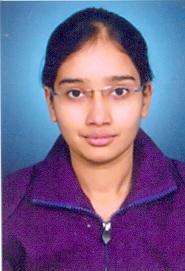
\includegraphics[scale=0.30]{Apoorva0006.jpg}
	\end{flushright}
\end{figure}
\textbf{OBJECTIVE:} 
To complete my project in given span of time with hardwork and dedication using my technical skills and knowledge and to learn new things and improve myself.
\newline

\textbf{EDUCATION:}

\begin{tabular}{|l|p{2in}|c|c|p{1in}|}
	\hline
	 \textbf{Degree} & \qquad \textbf{College/School} & \textbf{University/Board} & \textbf{Passing Year} & \textbf{Pass Percentage} \\
	\hline
	B.Tech & J.K Institute of Applied Physics and Technology & Allahabad University & $2017$(expected)) & $67.7$(upto ${1}^{st}$ year)\\
	\hline
	Intermediate & Sir Padampat Singhania Senior Secondary School & CBSE & $2012$ & \qquad $82.4$\\
	\hline
	High School & Sir Padampat Singhania Senior Secondary School & CBSE & $2010$ & $9.2$ CGPA\\
	\hline
\end{tabular}
\newline
\newline

\textbf{PROJECTS:}
\begin{enumerate}
	\item
    \item
\end{enumerate}

\textbf{TRAINING \& SEMINARS ATTENDED:}\\
\begin{tabular}{|p{2in}|p{2.5in}|c|p{1.3in}|}
	\hline
	\qquad \qquad \qquad \textbf{Event} & \qquad \qquad \qquad \textbf{Institution} & \textbf{Year} & \qquad \textbf{Key Learning}\\
	\hline
	Workshop on Robotics & Cepta InfoTech Pvt. Ltd at Motilal Nehru National Institute of Technology, Allahabad & $2013$ & Learned about basics of robotics\\
	\hline
	Workshop on html held at IETE & IETE & $2014$ & Project based learning in web designing\\
	\hline
	Seminar conducted by Dr. Sam Pitroda & Allahabad University & $2013$ & Motivation\\
	\hline
\end{tabular} 
\newline 
\newline

\textbf{RESEARCH PUBLICATIONS:}
\begin{enumerate}
	\item No research work done.
\end{enumerate}

\textbf{TECHNICAL SKILLS:}
\begin{itemize}
	\item C Programming
	\item Core Java
	\item Basic Web Designing
	\item Robotics
\end{itemize}
\newpage

\textbf{SOFT SKILLS:}
\begin{enumerate}
	\item Have lots of patience and determination 
	\item Always willing to learn new things and be innovative.
	\item Good team work as I am always supportive to others and try to convince others to work properly in a team.
\end{enumerate}

\textbf{EXTRA CURRICULAR ACTIVITIES:}
\begin{itemize}
	\item Secured $1^{st}$ position in basketball tournament in college basketball tournament.
	\item Secured first position in badmintion women singles at hostel fest.
	\item Runner Up in badminton at college fest, Avirbhav.
	\item Organized hostel fest of my hostel in Allahabad University.
\end{itemize}

\textbf{CO-CURRICULAR ACTIVITIES:}
\begin{enumerate}
	\item Winner at IIT BOMBAY, E-Yantra All India Robotics Competition 2012, Warehouse Managing Robot Theme
	Awarded for developing a warehouse managing robot for collecting and depositing the boxes based on the Firebird V Platform, sponsored by Ministry of Human Resource Development (MHRD), Govt. of India.
\end{enumerate}

\textbf{PERSONAL DETAILS:}
\begin{itemize}
	\item Father's Name: Mr Amit Bhargava
	\item Mother's Name: Mrs Jyotsna Bhargava
	\item Sex: Female
	\item Date of Birth: $13^{th}$ September $1994$
	\item Nationality: Indian
	\item Martial Status: Unmarried
\end{itemize}

\textbf{REFERENCE:}\\
Dr. N.K Shukla\\
Professor\\
Department of Electronics and Communication\\
University of Allahabad
\newline

\textbf{DECLARARION:}
I hereby certify that all the information provided above is true to the best of my knowledge.

\end{document}